\chapter{Results}

\section{SVD compression method results}

First example is an analysis of aging of nuclear power plant's containment made from prestressed concrete. The finite element mesh used in this analysis is in Figure \ref{fig:temelin:mesh}. More details about the analysis can be found in \cite{Kruis2012} and \cite{Koudelka2009}. This analysis includes high number of analysis time steps (thousands) with very little differences between them. There is therefore potential for compression to be very effective (compression ratio to be very low) as proven in Figure \ref{fig:temelin:NRMSD} that examines the impact of changes in the compression ratio to the mean error of approximation.

\begin{figure}[H]
\centering
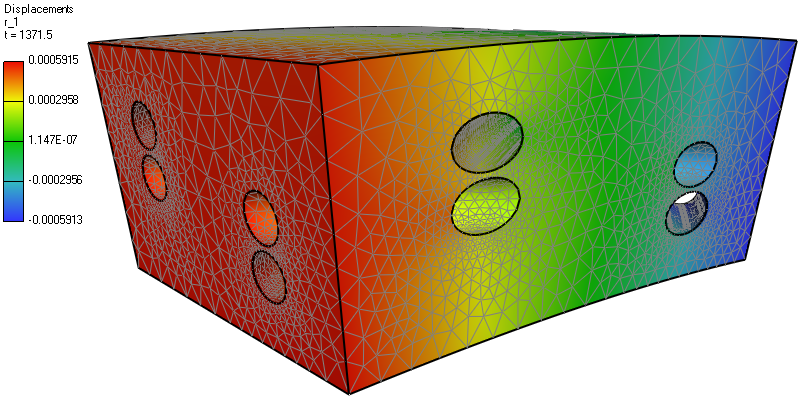
\includegraphics[width=\textwidth]{figures/chapter-SVD/temelin_screenshot}
\decoRule
\caption[Results visualization: reactor containment 3D.]{Segment of reactor containment analyzed. Results visualization (displacement field, x component).}
\label{fig:temelin:mesh}
\end{figure}

\begin{figure}[H]
\centering
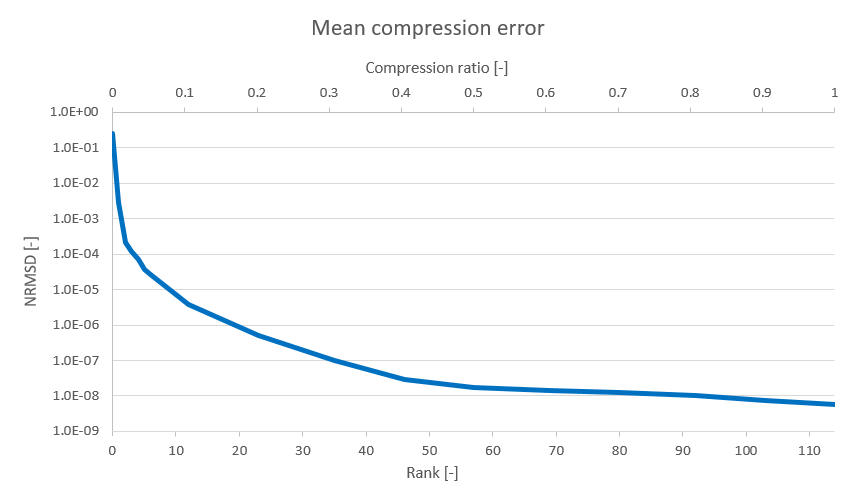
\includegraphics[width=\textwidth]{figures/chapter-SVD/temelin_NRMSD}
\decoRule
\caption[Dependence of NRMSD on compression ratio and rank (reactor containment 3D).]{Dependence of $\mathit{NRMSD}$ on $c$ and $r$ for reactor containment analysis results.} % ...$c$ (and $r$)...
\label{fig:temelin:NRMSD}
\end{figure}

% Execution times
Besides the error also the execution speed of compression algorithm was measured. In Figure \ref{fig:temelin:ExeTime}, there is a comparison of execution times for standard versus randomized SVD compression algorithms. Interestingly, execution time of standard SVD is independent of target rank whereas execution time of randomized SVD decreases linearly with decreasing target rank. If the rank is known ahead, the fact can be taken advantage of.

\begin{figure}[H]
\centering
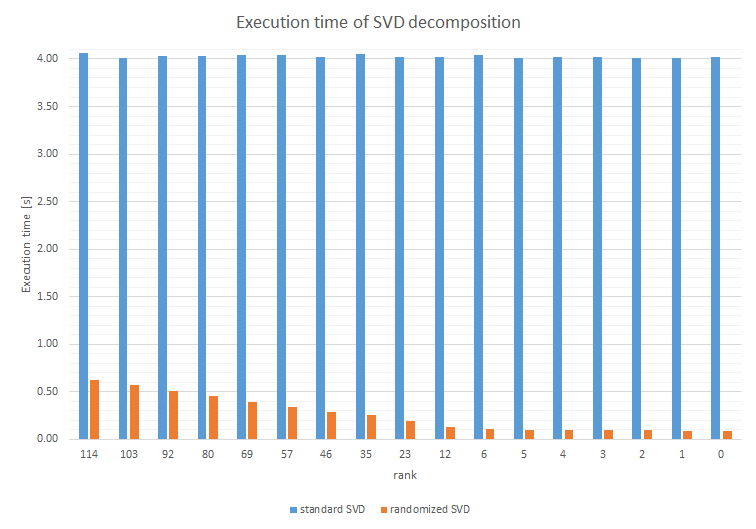
\includegraphics[width=\textwidth]{figures/chapter-SVD/temelin_ExecutionTime}
\decoRule
\caption[Execution time of standard and randomized SVD decompositions.]{Variation of execution time of standard and randomized SVD decompositions calculated for reactor containment analysis results.}
\label{fig:temelin:ExeTime}
\end{figure}

\section{Post-processor implementation results}

% Post-processors screenshots and description

This section contains screenshots and performance evaluation of both the desktop post-processor and the web post-processor. In Figure \ref{fig:desktop-postprocessor-remote-solutions}, there is a screenshot of the desktop post-processor that demonstrates the ability to connect to the remote web API and retrieve the list of solutions stored in the database.

\begin{figure}[H]
    \centering
    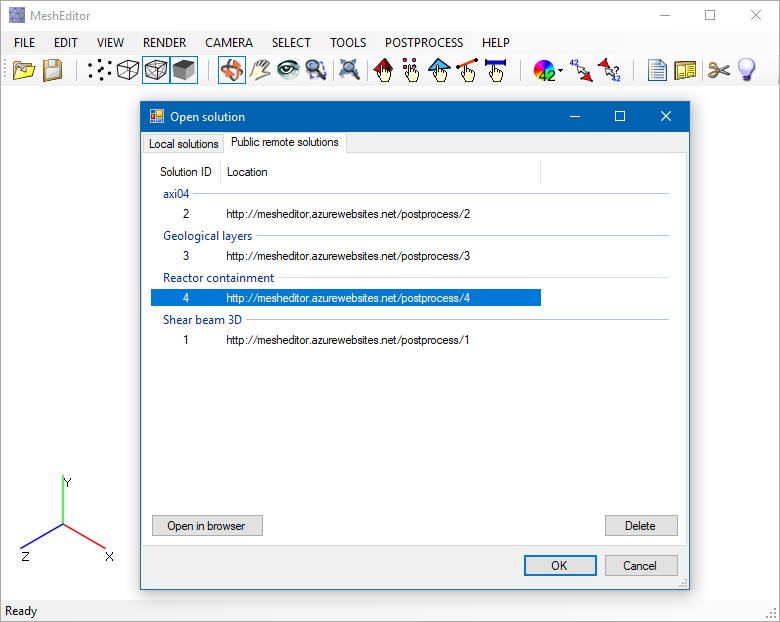
\includegraphics[width=\textwidth]{figures/chapter-data-management/desktop-postprocessor-remote-solutions}
    \decoRule
    \caption[Desktop post-processor screenshot. List of remote solutions.]{Desktop post-processor screenshot. Demonstration of connection to the web API (listing of remote solutions).}
    \label{fig:desktop-postprocessor-remote-solutions}
\end{figure}

Figure \ref{fig:desktop-postprocessor-master} shows the visualization of the master layer of the selected solution in the desktop post-processor window. The left panel contains the layer tree view that allows to choose the layers to show in the main window. There are also the options to visualize components of scalar, vector, or tensor data using the color scale on the mesh surface. Vector fields can be also visualized using arrows in the data locations pointing in the direction corresponding to the vector field. The top panel contains the tools for manipulation with the mesh, changing the camera view, selecting mesh entities, and assigning attributes to them.

\begin{figure}[H]
    \centering
    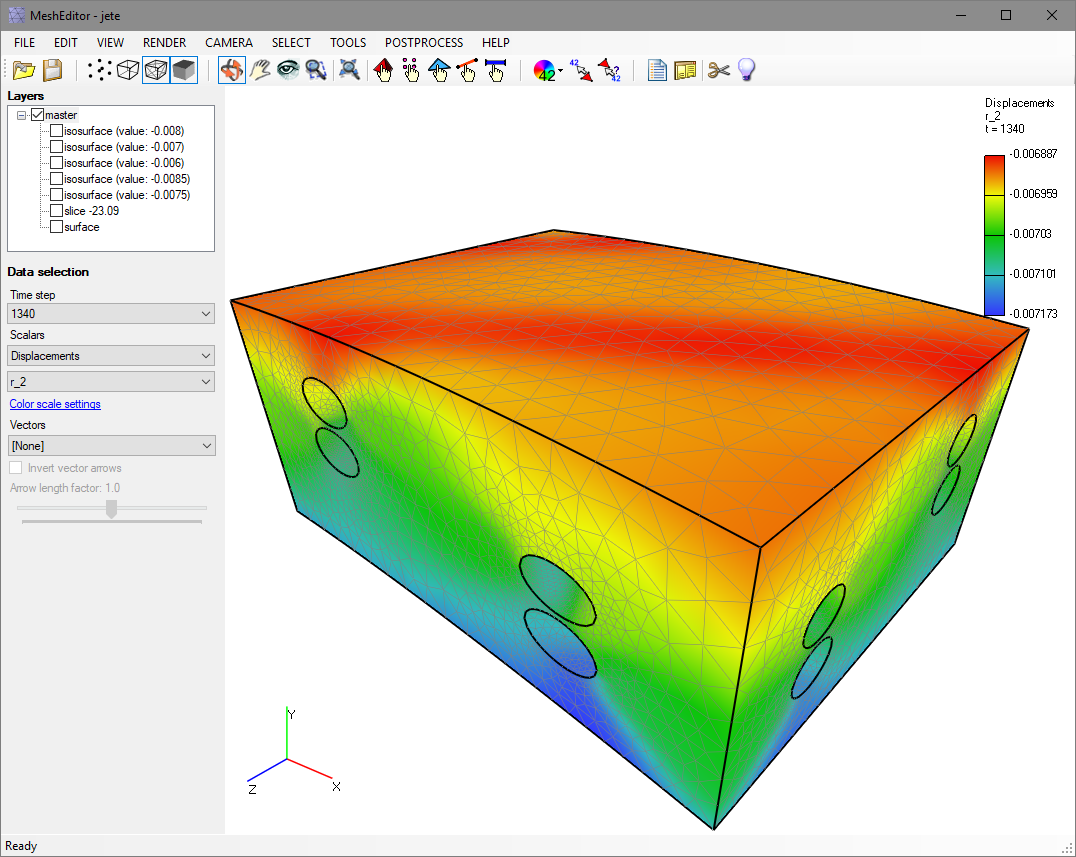
\includegraphics[width=\textwidth]{figures/chapter-data-management/desktop-postprocessor-master}
    \decoRule
    \caption{Desktop post-processor screenshot. Visualization of a master layer.}
    \label{fig:desktop-postprocessor-master}
\end{figure}

The post-processor also provides the user interface for definition of the parameters of a visual filter that the user wants to be applied on the selected layer. The parameters are sent as a part of the filter command that is sent to the FEM format converter component that generates the new layer. The layer tree is then updated and the new layer is displayed. The examples of slice and iso-surface layers are shown in Figure \ref{fig:desktop-postprocessor-slice} and Figure \ref{fig:desktop-postprocessor-isosurface}, respectively.

\begin{figure}[H]
    \centering
    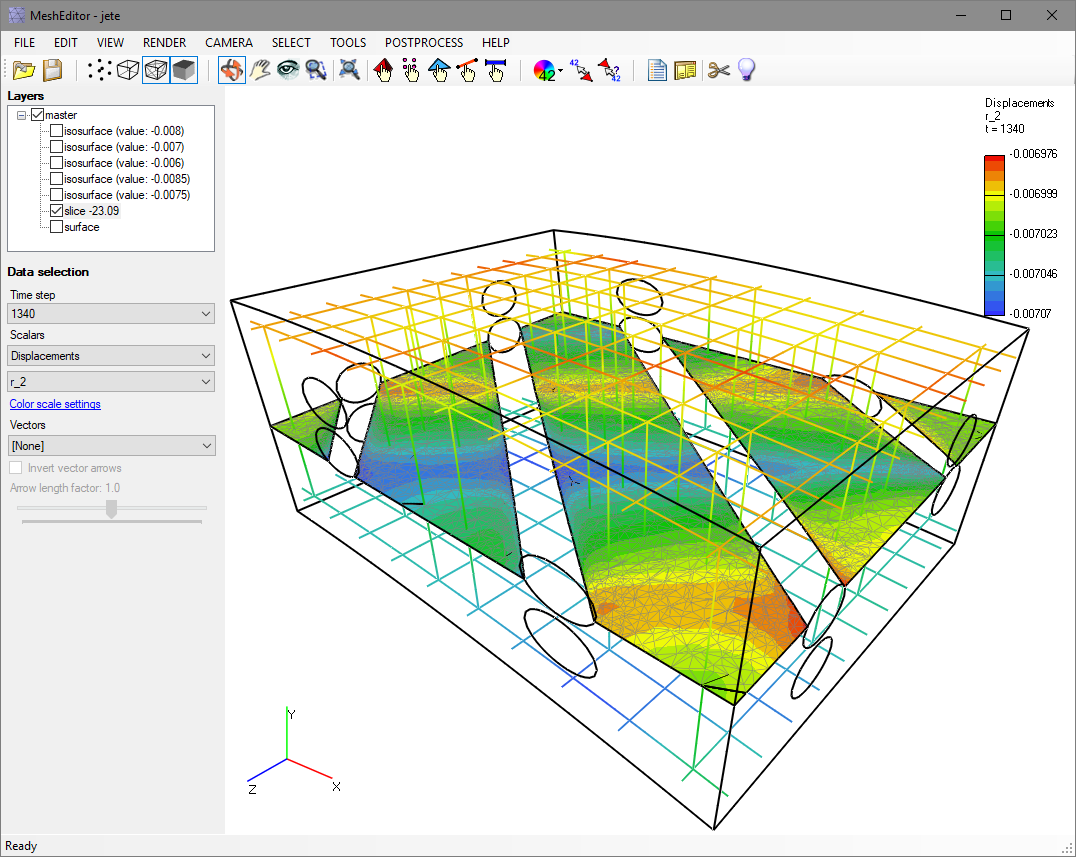
\includegraphics[width=0.85\textwidth]{figures/chapter-data-management/desktop-postprocessor-slice}
    \decoRule
    \caption{Desktop post-processor screenshot. Visualization of a slice layer.}
    \label{fig:desktop-postprocessor-slice}
\end{figure}

\begin{figure}[H]
    \centering
    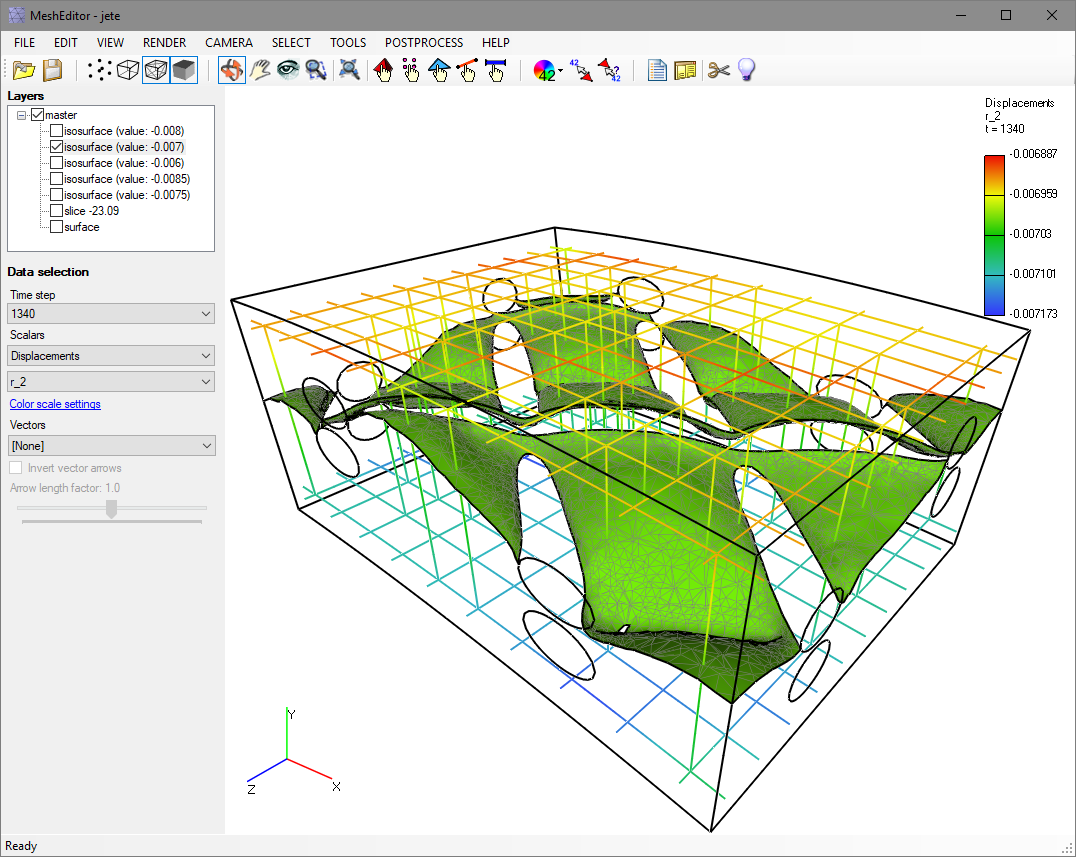
\includegraphics[width=0.85\textwidth]{figures/chapter-data-management/desktop-postprocessor-isosurface}
    \decoRule
    \caption{Desktop post-processor screenshot. Visualization of a iso-surface layer.}
    \label{fig:desktop-postprocessor-isosurface}
\end{figure}


\begin{figure}[H]
    \centering
    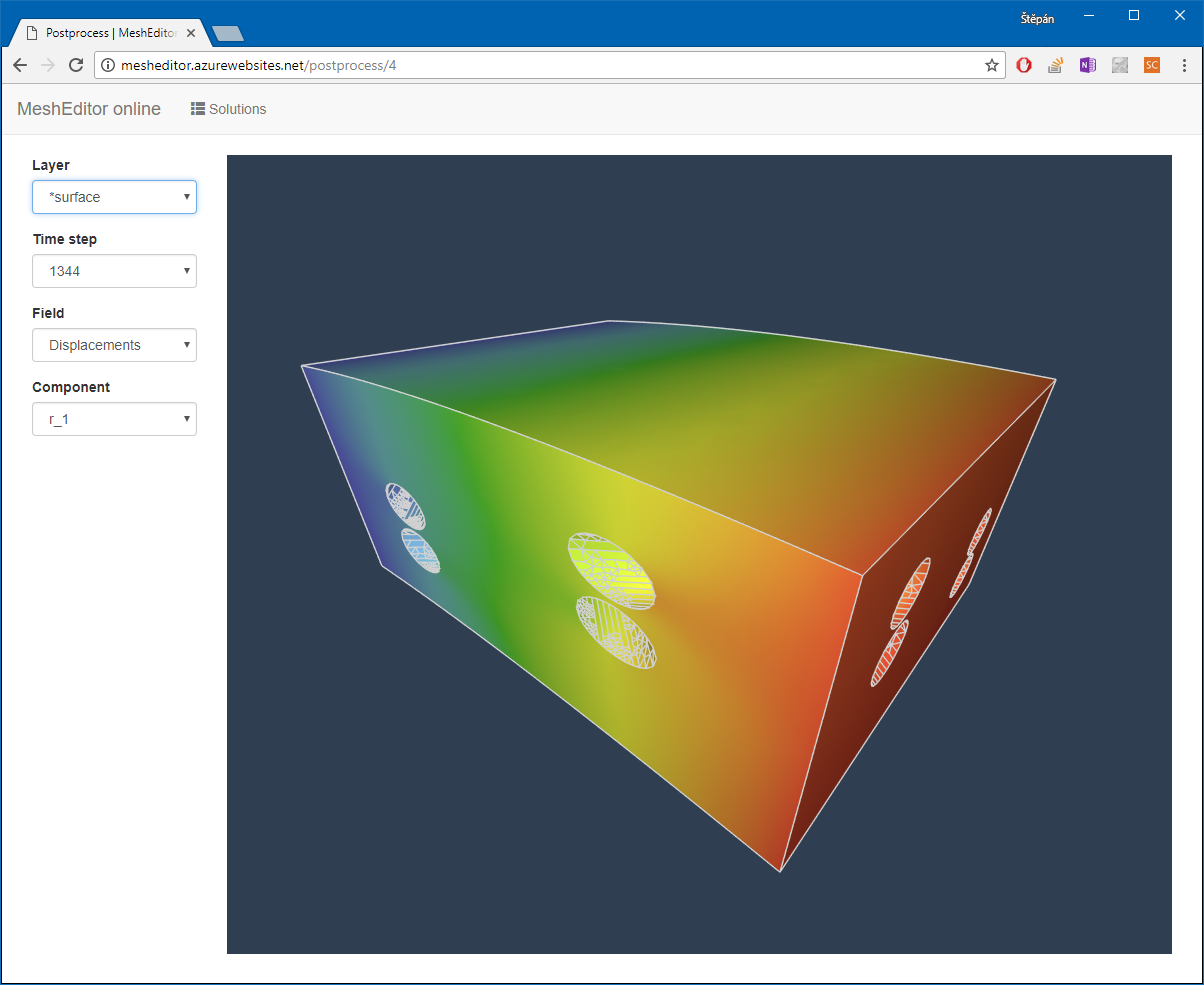
\includegraphics[width=0.75\textwidth]{figures/chapter-data-management/web-postprocessor-surface}
    \decoRule
    \caption{Web post-processor screenshot. Visualization of a surface layer.}
    \label{fig:web-postprocessor-surface}
\end{figure}

\begin{figure}[H]
    \centering
    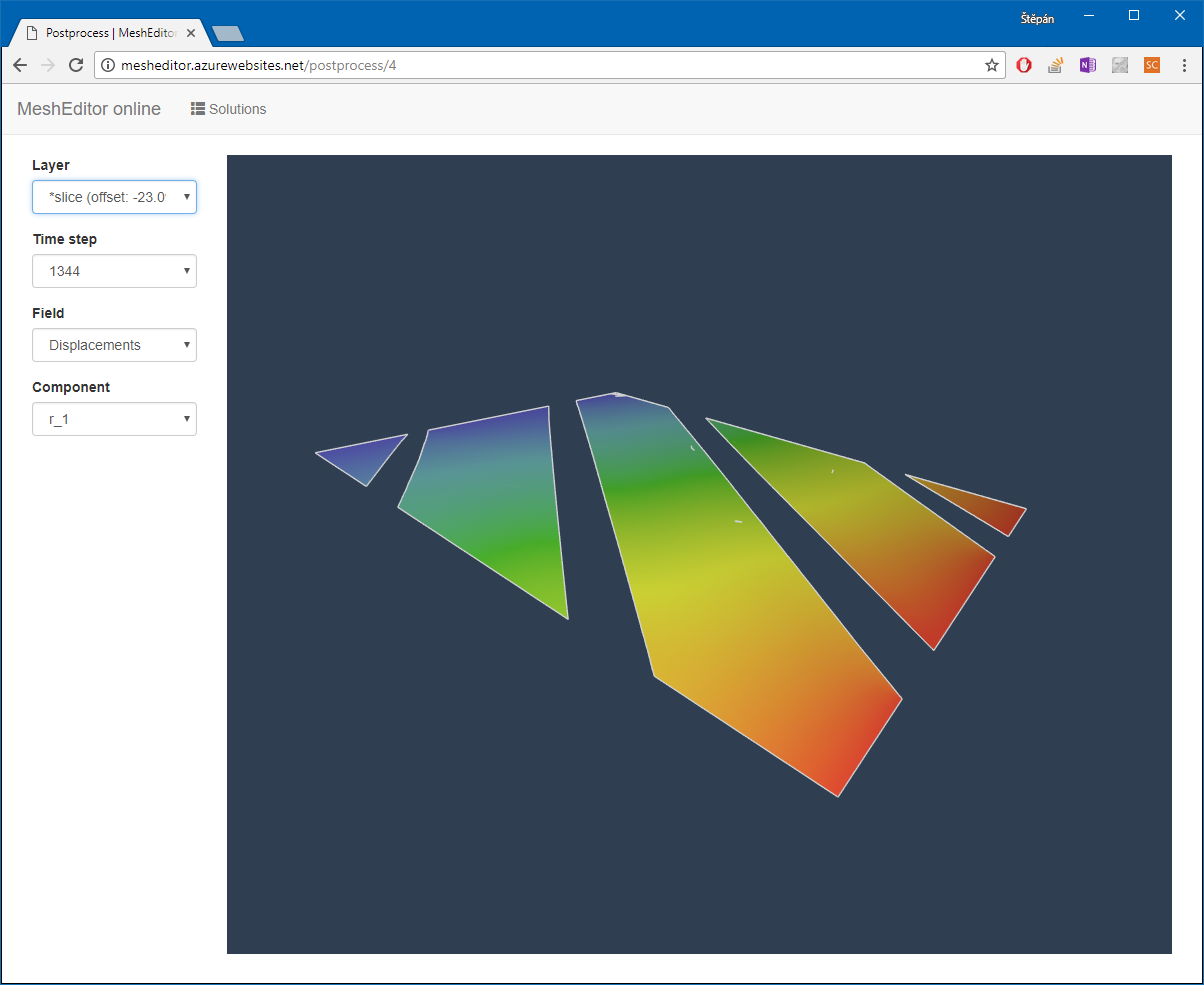
\includegraphics[width=0.75\textwidth]{figures/chapter-data-management/web-postprocessor-slice}
    \decoRule
    \caption{Web post-processor screenshot. Visualization of a slice layer.}
    \label{fig:web-postprocessor-slice}
\end{figure}

Figure \ref{fig:web-postprocessor-surface} shows the web post-processor that is connected to the same database as the desktop post-processor. The user interface also allows to select the layer of the current solution and the data component that should be visualized on the mesh surface. Figure \ref{fig:web-postprocessor-slice} contains the visualization of a slice layer.

\begin{figure}[H]
    \centering
    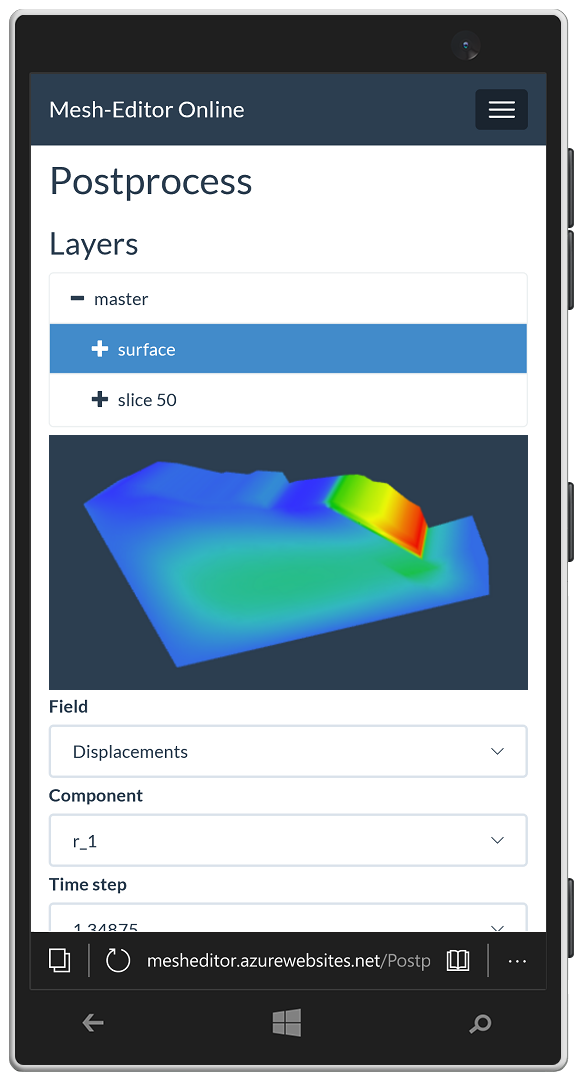
\includegraphics[width=0.35\textwidth]{figures/chapter-data-management/web-postprocessor-mobile}
    \decoRule
    \caption{Web post-processor screenshot taken on a mobile device.}
    \label{fig:web-postprocessor-mobile}
\end{figure}

Figure \ref{fig:web-postprocessor-mobile} demonstrates the fact that the web post-processor is fully capable of running on a mobile device with limited CPU and memory resources. The web application is designed to support multiple form factors and can be used comfortably even on a small device with touch screen.

Generation of a new filter layer is offloaded to the server and can took tens of seconds for large solutions. However, it is a one-time operation because the result is stored in a persistent storage. The subsequent requests for documents containing layer data are very fast. For a common mesh having around 300000 elements the web post-processor needs only tens of milliseconds to render layer geometry and selected data component on the mesh surface, even though it downloads all the necessary data from a remote server over the Internet. This speed allows to avoid caching of the data on the client device and helps to keep the memory consumption of the proposed post-processors very low (tens of megabytes for common mesh sizes) compared to traditional post-processors that need to load and process all the results from a file in order to display selected information.
